
\documentclass{article}

% ----------------------- PAQUETES ---------------------- %
% Set the font (output) encodings
\usepackage[T1]{fontenc}					% encoding de la fuente
\usepackage[spanish]{babel}				% paquete para los acentos en español
\usepackage{graphicx}							% paquete para poder usar graficos
\usepackage{float}								% paquete para poder usar \begin {figure}[H]
\usepackage{xurl}					% https://stackoverflow.com/questions/4146606/wrap-url-ignores-margin-in-bibtex-using-pdflatex
\usepackage{hyperref}							% paquete para hacer hyperreferencias a links
\usepackage{fancyhdr}							% paquete para poner cosas en footer y header
\usepackage{wrapfig}							% paquete para hacer wrapfigure
\usepackage{titling}							% paquete para modificar el espaciado de los titulos
\usepackage{titlesec}							% paquete para modificar como se ven los titulos
\usepackage{todonotes}						% paquete para hacer todos
\usepackage{subfiles}							% paquete para hacer subfiles


% ------------------------------------------------------- %

% ---------------------- CONFIGURACION ------------------ %

\graphicspath{{../informe/images}}
% ----------------- Configuracion de hyperref ----------- %
\hypersetup{								
	colorlinks=true,
	linkcolor=black,			%modo claro
	%linkcolor=white,		%modo oscuro
	filecolor=brown,		
	urlcolor=blue,
	pdftitle={Modelo de capacitación para uso de transporte público},
	}
% ------------------------------------------------------- %

% ----------------- Configuracion de fancyhdr --------------- %
\pagestyle{fancy}
\setlength{\headheight}{12.17pt} %esto esta para solucionar un warning del fancyhdr
\rfoot{Página \thepage}
\cfoot{}
\lfoot{Krapp Ramiro}
\renewcommand{\sectionmark}[1]{%
\markboth{\thesection\quad #1}{}}
\fancyhead[L]{\leftmark}
\fancyhead[R]{Modelo de transporte público}
\renewcommand{\headrulewidth}{2pt}
\renewcommand{\footrulewidth}{1pt}
% ------------------------------------------------------- %


%-------------- Formatos de los titulos --------------%
\newcommand{\sectionbreak}{\clearpage}
\titleformat{\section}
	{\bfseries \huge}
	{}
	{0em}
	{}[\titlerule]

\titleformat{\subsection}
	{\bfseries \Large}
	{}
	{0em}
	{}

\titleformat{\subsubsection}
	{\bfseries \large}
	{}
	{0em}
	{}

\titlespacing{\section} %me permite controlar el espaciado de la seccion que le indico
	{0em}
	{0em}
	{1.5em}

\titlespacing{\subsection}
{0em} %sangria
{3em} %separacion con lo que hay arriba
{0.5em} %separacion con lo que hay abajo
%----------------------------------------------------- %

% ----------------- FIN DE CONFIGURACION ------------- %

\begin{document}

\begin{titlepage}
	\begin{center}
		\vspace{1cm}

		{\Huge
			\textbf{Modelo de capacitación para uso de transporte público}}

		\vspace{0.3cm}
		{\LARGE
			Informe técnico}

		\vspace{0.5cm}
		{\Large
			Un trabajo presentado para la materia de \\
			Emprendimiento Local y Desarrollo Productivo}

		\vspace{2cm}

		\begin{figure}[H]
			\centering
			
\includegraphics[width=0.6\textwidth]{logo.png}
		\end{figure}

		\vfill

		{\Large
			\textbf{Krapp Ramiro} \\
			\vspace{0.5cm}
			Instituto tecnológico San Bonifacio\\
			Departamento de electrónica\\
			\today
		}

		\vspace{0.5cm}
		{\large Hecho en {\LaTeX}\\
			Versión Alpha 0.1}

	\end{center}
\end{titlepage}

\section{Introducción}
El modelo de capacitación para uso de transporte público es un modelo \todo{es redundante}
del sistema de transporte público ferroviario de la provincia de Buenos Aires,
diseñado para capacitar a alumnos de primaria, para que aprendan a transportarse
emulando el sistema de tarjeta SUBE / molinillo.

Este está pensado para ser presentado en escuelas primarias, con el objetivo de
que los alumnos aprendan en un espacio controlado cómo funciona el transporte público,
para que tengan la capacidad de desarrollarse a futuro en la vida adolescente y adulta

Este modelo presenta un sistema de multiples lectores RFID, los cuales
emulan los lectores de tarjeta que se presentan en múltiples ámbitos, como el sistema
de trenes, el sistema de colectivos, el sistema de transporte subterraneo, etc\ldots.

Tambien presenta un set de tarjetas y llaveros, los cuales emulan la propia tarjeta,
y con los cuales los alumnos aprenderán conceptos tales como el pago usando la misma,
el recargo de saldo, etc\ldots
\vspace{2em}

\begin{figure}[H]
	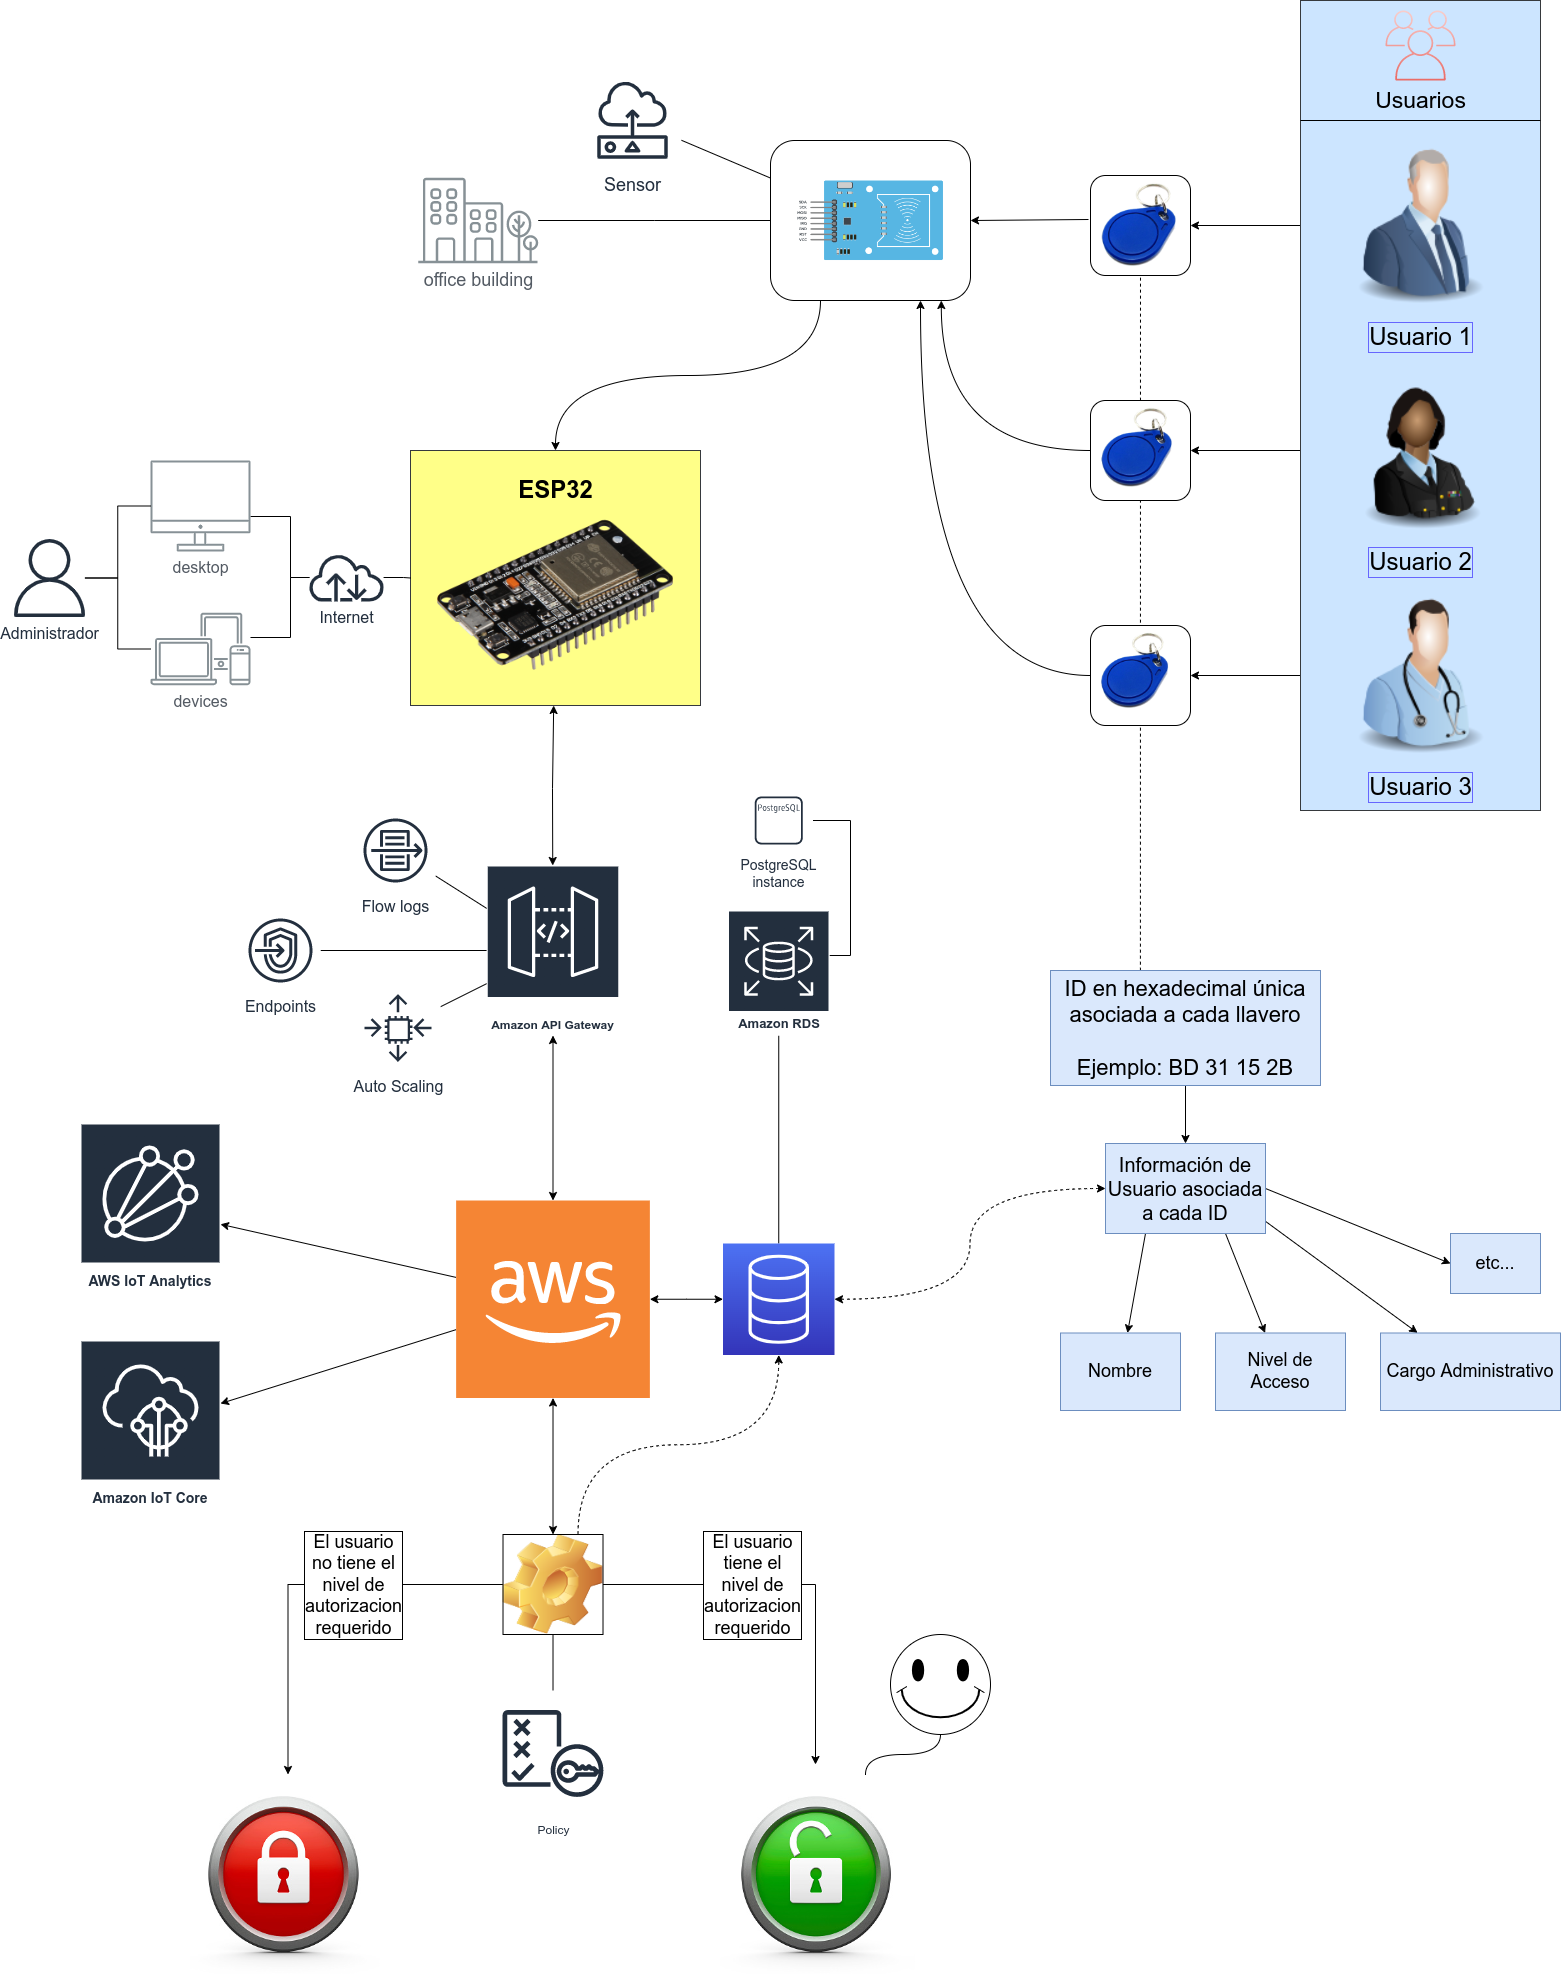
\includegraphics[width=\textwidth]{diagrama.drawio.png}
	\centering
	\caption{Un diagrama del modelo}
\end{figure}
\end{document}